\documentclass[a4paper,ngerman,12pt]{scrartcl}

\usepackage[utf8]{inputenc}
%\usepackage[ansinew]{inputenc}

\usepackage[ngerman]{babel}

\usepackage{amsmath,amsthm,amssymb,stmaryrd,color,graphicx}
\usepackage{setspace}
\usepackage{bussproofs}
\usepackage{array}
\usepackage{comment}
\usepackage{wrapfig}

\usepackage{enumitem}

\usepackage{units}

\usepackage[protrusion=true,expansion=true]{microtype}

\usepackage{lmodern}

\usepackage{hyperref}
\usepackage{cleveref}

\newcommand{\RR}{\mathbb{R}}
\newcommand{\CC}{\mathbb{C}}
\newcommand{\ZZ}{\mathbb{Z}}
\newcommand{\NN}{\mathbb{N}}
\newcommand{\QQ}{\mathbb{Q}}

\setlength\parskip{\medskipamount}
\setlength\parindent{0pt}

\theoremstyle{definition}
\newtheorem{defn}{Definition}[]
\newtheorem{axiom}[defn]{Axiom}
\newtheorem{bsp}[defn]{Beispiel}

\RequirePackage{framed}
\newtheorem{aufg}{Aufgabe}
\definecolor{shadecolor}{rgb}{.96,.96,.96}
\newenvironment{aufgabe}[1][]
		{\begin{shaded}\vspace{-0.3cm}\begin{aufg}\emph{#1} \par\medskip}
		{\end{aufg}\vspace{-0.3cm}\end{shaded}}


\theoremstyle{plain}
\newtheorem{prop}[defn]{Proposition}
\newtheorem{motto}[defn]{Motto}
\newtheorem{wunder}[defn]{Wunder}
\newtheorem{ueberlegung}[defn]{Überlegung}
\newtheorem{lemma}[defn]{Lemma}
\newtheorem{kor}[defn]{Korollar}
\newtheorem{hilfsaussage}[defn]{Hilfsaussage}
\newtheorem{satz}[defn]{Satz}
\newtheorem{frage}[defn]{Frage}

\theoremstyle{remark}
\newtheorem{bem}[defn]{Bemerkung}

	
\newtheorem*{antwort}{Antwort}

%\newlength{\aufgabenskip}
%\setlength{\aufgabenskip}{1.4em}
%\newcounter{aufgabennummer}
%\newenvironment{aufgabe}[1]{
%	\addtocounter{aufgabennummer}{1}
%	\textbf{Aufgabe \theaufgabennummer.} \emph{#1} \par
%}{\vspace{\aufgabenskip}}

\clubpenalty=10000
\widowpenalty=10000
\displaywidowpenalty=10000

\setlength\unitlength{1cm}

\usepackage{tikz}
\usetikzlibrary{calc}
\usepackage{adjustbox}
\usepackage{algorithm2e}

\RequirePackage{geometry}
\geometry{textwidth=16.0cm,textheight=24.5cm,footskip=1.5cm}


\newcommand{\kante}[2]{#1{-}#2}
\newcommand{\edge}[3]{\draw[thick] (#1) --node[rectangle,fill=gray!10]{$#3$} (#2);}

\begin{document}
	
\begin{picture}(0,0)
\put(0,-0.5){%
	
\includegraphics[scale=0.1]{logo-ifm}
}
\put(14.0,-3.5){%
	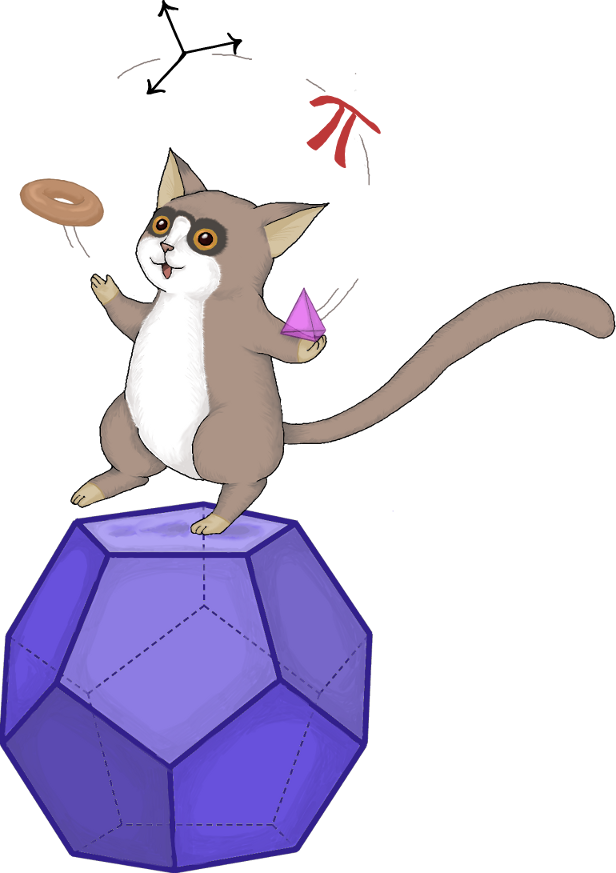
\includegraphics[scale=0.17]{cover}
}
\end{picture} 
	
\vspace{6em}

\begin{center}\Large{Mai-Mathetag 2022}

\section*{Kürzeste Wege berechnen}\end{center}

In diesem Brief wollen wir uns damit beschäftigen wie man kürzeste Wege berechnen kann -- wir wollen uns also damit beschäftigen wie man (mathematisch) Fragestellungen der folgenden Form beantworten kann:

Wir sind am Augsburger Hauptbahnhof und möchten gerne zum Roten Tor. Was ist der kürzeste Weg dorthin?

\begin{center}
	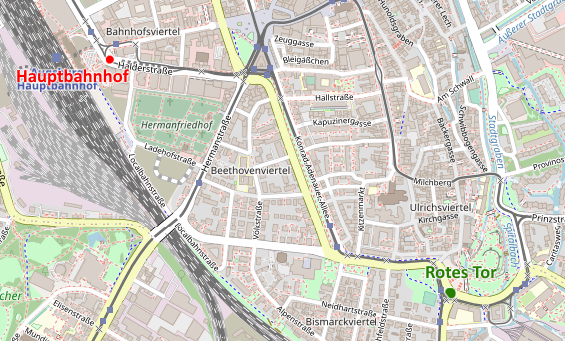
\includegraphics[width=.5\textwidth]{bilder/StadtplanAugsburg.png}\\
	\tiny{Ein Ausschnitt aus dem Augsburger Stadtplan © OpenStreetMap-Mitwirkende}
\end{center}

Wie würdest du laufen? Warum glaubst du, dass das der kürzeste Weg ist? Und wie hast du diesen Weg gefunden? Bist du dir sicher, dass es der kürzeste Weg ist?

Wie du vielleicht schon merkst, lassen sich diese Fragen so nicht wirklich mathematisch präzise beantworten. Wir müssen also erstmal noch das Problem etwas präziser formulieren. Als ersten Schritt wollen wir dazu den echten Stadtplan durch ein etwas übersichtlicheres Bild ersetzen:

\begin{center}
	\begin{tikzpicture}[scale=.8]
		\node[draw,circle](s) at (0,0) {Hbf};
		\node[draw,circle](1) at (4,0) {$1$};
		\node[draw,circle](2) at (8,0) {$2$};
		\node[draw,circle](3) at (0,-3) {$3$};
		\node[draw,circle](4) at (3,-3) {$4$};
		\node[draw,circle](5) at (2,-6) {$5$};
		\node[draw,circle](6) at (6,-4) {$6$};
		\node[draw,circle](7) at (7,-6) {$7$};
		\node[draw,circle](8) at (10,-4) {$8$};
		\node[draw,circle](9) at (10,-6) {$9$};
		\node[draw,circle](t) at (13,-7) {Tor};
		
		\edge{s}{1}{3}	
		\edge{s}{3}{2}
		\edge{1}{2}{4}	
		\edge{1}{4}{3}
		\edge{1}{6}{5}
		\edge{2}{8}{6}
		\edge{3}{4}{2}
		\edge{3}{5}{2}
		\edge{4}{5}{1}
		\edge{4}{6}{3}
		\edge{5}{7}{6}
		\edge{6}{7}{2}
		\edge{6}{8}{4}
		\edge{7}{9}{3}
		\edge{8}{9}{4}
		\edge{8}{t}{8}
		\edge{9}{t}{1}
	\end{tikzpicture}
\end{center}

In diesem Bild haben wir die Straßen durch gerade Linien und die Kreuzungen durch Kreise dargestellt.\footnote{Damit das Bild nicht zu unübersichtlich wird habe ich zudem auch noch einige Straßen weggelassen.} Außerdem haben wir auf jede Linie eine Zahl geschrieben -- diese soll aussagen wie lang diese Straße ist, das heißt wie lange man von einer Kreuzung zur nächsten braucht. 

So ein Bild nennt man in der Mathematik auch einen \emph{Graphen}. Die Linien nennt man dann \emph{Kanten} und die Kreise \emph{Knoten}. Ein Weg ist jetzt einfach eine Abfolge von Kanten -- beispielsweise ist $\mathrm{Hbf} \rightarrow 1 \rightarrow 4 \rightarrow 6 \rightarrow 8 \rightarrow \mathrm{Tor}$ ein möglicher Weg vom Hauptbahnhof zum Roten Tor (in unserem Graphen) und hat eine Länge von $3+3+3+4+8=21$. Unsere Aufgabe ist es jetzt einen \emph{kürzesten} solchen Weg in dem Graphen zu finden.

Was meinst du? Ist das schon ein kürzester Weg? Oder findest du noch einen kürzeren Weg? 

Tatsächlich ist unser aktueller Weg noch nicht optimal. Das können wir besonders einfach daran sehen, dass wir einen kürzeren Weg erhalten, indem wir eine Abkürzung gehen: Statt von $8$ direkt zum Tor zu gehen, können wir über den Knoten $9$ laufen -- statt einer Länge von $8$ haben wir dann nur noch eine Länge von $4+1=5$. 

\begin{center}
	\begin{adjustbox}{max width=.45\textwidth}
		\begin{tikzpicture}[scale=.8]
			\node[draw,circle](s) at (0,0) {Hbf};
			\node[draw,circle](1) at (4,0) {$1$};
			\node[draw,circle](4) at (3,-3) {$4$};
			\node[draw,circle](6) at (6,-4) {$6$};
			\node[draw,circle](8) at (10,-4) {$8$};
			\node[draw,circle](t) at (13,-7) {Tor};
			
			\edge{s}{1}{3}	
			\edge{1}{4}{3}
			\edge{4}{6}{3}
			\edge{6}{8}{4}
			\edge{8}{t}{8}
		\end{tikzpicture}
	\end{adjustbox}
	\hfill
	\begin{adjustbox}{max width=.45\textwidth}
		\begin{tikzpicture}[scale=.8]
			\node[draw,circle](s) at (0,0) {Hbf};
			\node[draw,circle](1) at (4,0) {$1$};
			\node[draw,circle](4) at (3,-3) {$4$};
			\node[draw,circle](6) at (6,-4) {$6$};
			\node[draw,circle](8) at (10,-4) {$8$};
			\node[draw,circle](9) at (10,-6) {$9$};
			\node[draw,circle](t) at (13,-7) {Tor};
			
			\edge{s}{1}{3}	
			\edge{1}{4}{3}
			\edge{4}{6}{3}
			\edge{6}{8}{4}
			\edge{8}{9}{4}
			\edge{9}{t}{1}
		\end{tikzpicture}
	\end{adjustbox}
\end{center}

Auf diese Weise können wir jetzt immer weitermachen: Wir schauen, ob wir irgendwo eine Abkürzung finden und wenn ja, dann nehmen wir diese (und machen unseren Weg so kürzer). Das machen wir so lange, bis wir keine Abkürzung mehr finden. Und dann? Haben wir dann einen kürzesten Weg gefunden? 

Dazu müssten wir uns ganz sicher sein, dass es keine weitere Abkürzung mehr gibt (dass wir also keine übersehen haben). Das klingt sehr schwierig das zu überprüfen. Insbesondere könnte eine Abkürzung ja auch ein völlig anderer (kürzerer) Weg sein! im Grunde müssen wir also \emph{alle möglichen Wege} durchprobieren und schauen, welcher davon der kürzeste ist. Nur wenn wir das machen, können wir uns wirklich sicher sein, den kürzesten Weg gefunden zu haben. Aber ist das überhaupt machbar? Alle Wege durchprobieren?

\begin{aufgabe}\label{aufg:WegeZahlen}
	Wie viele mögliche Wege gibt es in unserem Graphen?
	\begin{enumerate}[label=\alph*)]
		\item Was schätzt du: Wie viele verschiedene Wege vom Hauptbahnhof zum Roten Tor gibt es in unserem Graphen?
		\item Nehmen wir einmal kurz an, jeder der $12$ Knoten wäre mit jedem anderen Knoten durch eine direkte Kante verbunden (das nennt man dann einen \emph{vollständigen Graphen}). Wie viele Wege vom Hauptbahnhof zum Roten Tor gäbe es dann? Das ist eine obere Schranke an die Anzahl der Wege in unserem tatsächlichen Graphen. Warum?\\
		\textbf{Hinweis:} Du darfst hier annehmen, dass ein Weg sinnvollerweise nie zweimal über die gleiche Kreuzung läuft. Bestimme jetzt wie viele Wege aus $1$ Kante es gibt. Wie viele Wege aus $2$ Kanten. Wie viele Wege aus $3$ Kanten. Usw.
		\item Nehmen wir nun stattdessen an die $12$ Knoten wären in einem $3\times 4$-Gitter angeordnet, wobei unser Startknoten ganz links oben und unser Zielknoten ganz rechts unten ist. Wie viele Wege gibt es jetzt, bei denen wir immer nur entweder nach rechts oder nach unten laufen? Das ist eine untere Schranke an die Gesamtzahl der Wege in unserem Gittergraphen. Warum?
		\item Stell dir nun vor wir hätten einen Gittergraphen mit $10\times 10$ Knoten. Was sind die untere und obere Schranke nun? Was ist mit einem $n \times n$ Gitter?
	\end{enumerate}
\end{aufgabe}

Offenbar ist es also nicht sinnvoll alle Wege durchzuprobieren! Wir brauchen daher ein sinnvolleres systematisches Verfahren: Einen \emph{Algorithmus}! Ein Algorithmus ist dabei im Grunde nichts anderes als eine Zerlegung eines großen, komplexen Problems in viele kleine und einfach zu lösende Teilprobleme. 

Im Folgenden werden wir zwei Algorithmen für das Kürzeste-Wege-Problem kennen lernen(es gibt natürlich noch viel mehr!)

\section{Der Algorithmus von Bellman-Ford}

Weil sich die Algorithmen so leichter erklären lassen, werden wir im Folgenden die Problemstellung leicht abwandeln: Wir bekommen weiterhin einen Graphen mit einem festen Startknoten (den wir ab sofort $s$ nennen werden) gegeben. Statt aber nun einen konkreten kürzesten Weg zu einem festen Endknote zu bestimmen, wollen wir erstmal nur für jeden Knoten des Graphen seine \emph{Distanz} vom Startknoten $s$ bestimmen (also die Länge eines kürzesten Weges vom Startknoten zu diesem Knoten). Für einen Knoten $v$ werden wir diese Distanz mit $d(v)$ bezeichnen (in unserem Augsburg-Graphen gilt also zum Beispiel $d(3)=2$).

Der Algorithmus von Bellman und Ford basiert nun im Wesentlichen auf unserer Abkürzungsidee von vorhin: Wir starten mit \glqq irgendwelchen\grqq{} Distanzen $\tilde{d}(v)$, für die wir uns sicher sind, dass wir die Knoten in dieser Zeit (oder schneller) erreichen können. Dann schauen wir immer wieder, ob es noch irgendwo eine Abkürzung gibt, durch die wir $\tilde{d}$ kleiner machen können. Das wollen wir dann so lange machen, bis wir uns sicher sein können, dass wir alle Abkürzungen gefunden haben.

Das ist jetzt aber natürlich immer noch etwas vage. Darum wollen wir die einzelnen Schritte jetzt genauer erklären:
\begin{itemize}
	\item Als Startwerte können wir $\tilde{d}(s) = 0$ und $\tilde{d}(v) = \infty$ für alle anderen Knoten $v$ wählen. Denn den Startknoten erreichen wir natürlich in $0$ Zeit -- und alle anderen sicher in unendlich Zeit (oder -- hoffentlich -- schneller).
	\item Statt alle nur möglichen Abkürzungen anzuschauen, betrachten wir nur Abkürzungen über einzelne Kanten. Wenn wir eine Kante $\kante{v}{w}$ (also eine Kante zwischen den Knoten $v$ und $w$) haben, dann prüfen wir ob wir den Knoten $w$ schneller erreichen können, indem wir zuerst zu $v$ und dann von dort über die Kante $\kante{v}{w}$ zu $w$ gehen. Falls dem so ist, passen wir $\tilde{d}(w)$ entsprechend an. Falls nicht, ändert sich nichts. Dann machen wir das gleiche mit vertauschten Rollen von $v$ und $w$.
\end{itemize}

Ist dir klar, warum die obigen beiden Schritte korrekt sind? Warum gilt hier also zu jedem Zeitpunkt, dass es für jeden Knoten $v$ einen Weg von $s$ zu $v$ gibt, dessen Länge höchstens $\tilde{d}(v)$ ist?

Wenn wir das verstanden haben, bleibt nur noch die Frage, wie oft wir diesen Abkürzungsschritt machen müssen, damit wir die tatsächlichen Distanzen bestimmt haben (also damit $\tilde{d}(v)=d(v)$ gilt)? Die Antwort auf diese Frage liefert der folgende Satz:

\begin{satz}
	Sei $s{-}v_1{-}v_2{-}v_3{-}\dots{-}v_k$ ein kürzester Weg von $s$ nach $v_k$. Wenn wir (in dieser Reihenfolge, aber möglicherweise noch mit anderen Schritten dazwischen) die Kanten $\kante{s}{v_1}, \kante{v_1}{v_2}, \kante{v_2}{v_3}, \dots, \kante{v_{k-1}}{v_k}$ betrachten (und gegebenenfalls abkürzen), dann gilt danach $\tilde{d}(v_k) = d(v_k)$.
\end{satz}

\begin{aufgabe}
	Zeige, dass dieser Satz richtig ist.
	
	\textbf{Tipp:} Zeige zunächst die folgende (einfachere) Aussage: Gilt $\tilde{d}(v) = d(v)$ und wir machen einen Abkürzungsschritt zur Kante $\kante{v}{w}$, dann gilt danach auch $\tilde{d}(w) = d(w)$. Überlege dir dann wie daraus der obige Satz folgt.
\end{aufgabe}

Mit diesem Satz können wir uns jetzt leicht überlegen wie oft wir Abkürzungsschritte ausführen müssen: Nehmen wir an unser Graph hat $n$ Knoten. Dann besteht ein kürzester Weg sicher nicht aus mehr als $n-1$ Kanten (warum?). Zusammen mit dem obigen Satz folgt daraus, dass wir fertig sind, wenn wir $(n-1)$-mal jede Kante für einen Abkürzungsschritt betrachtet haben. Kannst du erkennen, warum das so ist?

Der vollständige Algorithmus lautet nun wie folgt:
 
\begin{algorithm}
	\KwIn{Ein Graph mit Längenangaben auf den Kanten und ein Startknoten $s$}
	\KwOut{Für jeden Knoten $v$ dessen Distant $d(v)$ von $s$ aus}
	
	Setze $\tilde{d}(s) = 0$ und $\tilde{d}(v) = \infty$ für alle knoten $v \neq s$
	
	\For{$i = 1, 2, \dots, n-1$}{
		\ForEach{Kante $v-w$}{
			\If{$\tilde{d}(v) + \text{ Länge von } \kante{v}{w} < \tilde{d}(w)$}{
				Setze $\tilde{d}(w) = \tilde{d}(v) + \text{ Länge von } \kante{v}{w}$
			}
			\If{$\tilde{d}(w) + \text{ Länge von } \kante{w}{v} < \tilde{d}(v)$}{
				Setze $\tilde{d}(v) = \tilde{d}(w) + \text{ Länge von } \kante{w}{v}$
			}
		}
	}
\end{algorithm}

\begin{aufgabe}
	Führe den Algorithmus von Bellman-Ford auf dem Beispiel-Graphen vom Anfang aus.
\end{aufgabe}

\begin{aufgabe}\label{aufg:LaufzeitBF}
	Wie oft musst du für unseren Beispiel-Graphen einen Abkürzungsschritt durchführen? 
	
	Wie oft müsstest du das bei einem Graphen aus $n$ Knoten (höchstens) machen? Vergleiche dein Ergebnis mit dem aus Aufgabe 1.
\end{aufgabe}

\section{Der Algorithmus von Dijkstra}

Wir wir gesehen haben, ist der Algorithmus von Bellman-Ford deutlich schneller als einfach alle möglichen Wege durchzuprobieren. Allerdings ist er oft immer noch ziemlich ineffizient: So kommt es oft vor, dass wir die gleiche Kante immer wieder anschauen, ohne dadurch noch eine Abkürzung zu finden. Hier wäre es sehr hilfreich, wenn wir wüssten, wann wir mit einer bestimmten Kante fertig sind (diese also im weiteren Verlauf nicht mehr betrachten müssen). Der folgende Satz gibt uns einen sehr nützlichen Trick dafür:

\begin{satz}\label{satz:DijkstraKnotenFertig}
	Sei $v$ ein Knoten, für den $\tilde{d}(v) = d(v)$ gilt (wir kennen also bereits seine wahre Distanz vom Startknoten). Führen wir noch einen Abkürzungsschritt mit der Kante $\kante{v}{w}$ durch, so werden wir danach nie wieder eine Abkürzung über diese Kante finden.
\end{satz}

\begin{aufgabe}
	Zeige, dass der obige Satz wirklich wahr ist.
\end{aufgabe}

Jetzt wissen wir also, welche Kanten wir im Laufe des Algorithmus nicht mehr weiter betrachten müssen. Wir müssen nur noch herausfinden, für welche Knoten bereits $\tilde{d}(v) = d(v)$ gilt. Fällt dir ein Knoten ein, für den das bereits am Anfang des Algorithmus gilt?

Für unseren verbesserten Algorithmus werden wir die Knoten in zwei Gruppen einteilen -- die fertigen Knoten und die unfertigen. Die fertigen Knoten sollen dabei die Eigenschaft haben, dass für sie bereits $\tilde{d}(v) = d(v)$ gilt und wir für jede mit ihnen verbundene Kante bereits den letzten Abkürzungsschritt gemacht haben. Wegen dem obigen Satz wissen wir dann, dass wir alle Kanten, die von einem fertigen Knoten ausgehen, im Weiteren ignorieren können. Diese Überlegung führt uns zum folgenden Algorithmus von Dijkstra:

\begin{algorithm}
	\KwIn{Ein Graph mit Längenangaben auf den Kanten und ein Startknoten $s$}
	\KwOut{Für jeden Knoten $v$ dessen Distant $d(v)$ von $s$ aus}
	
	Setze $\tilde{d}(s) = 0$ und $\tilde{d}(v) = \infty$ für alle knoten $v \neq s$
	
	Nenne alle Knoten \glqq unfertig\grqq
	
	\While{es gibt noch unfertige Knoten}{
		Wähle einen unfertigen Knoten $v$ mit geringstem $\tilde{d}(v)$ unter allen unfertigen Knoten.
		
		\ForEach{Kante $v-w$, die von $v$ ausgeht}{
			\If{$\tilde{d}(v) + \text{ Länge von } \kante{v}{w} < \tilde{d}(w)$}{
				Setze $\tilde{d}(w) = \tilde{d}(v) + \text{ Länge von } \kante{v}{w}$
			}
			\If{$\tilde{d}(w) + \text{ Länge von } \kante{w}{v} < \tilde{d}(v)$}{
				Setze $\tilde{d}(v) = \tilde{d}(w) + \text{ Länge von } \kante{w}{v}$
			}
		}
	
		Nenne den Knoten $v$ \glqq fertig\grqq
	}
\end{algorithm}

\begin{aufgabe}
	Überzeuge dich, dass der obige Algorithmus wirklich korrekt ist.
	
	\textbf{Hinweis:} Einen vollständigen Beweis hierfür zu finden, ist nicht ganz einfach. Aber vielleicht bist du ja schon davon überzeugt, dass der Algorithmus korrekt ist, wenn du die folgenden Fragen beantworten kannst:
	\begin{itemize}
		\item Warum kann sich der Wert $\tilde{d}(v)$ eines Knotens $v$ nicht mehr ändern, nachdem wir ihn als fertig bezeichnet haben.
		\item Warum gilt für alle fertigen Knoten $v$, dass wir bereits ihre wahre Distanz von $s$ kennen also ($\tilde{d}(v)=d(v)$)?
		\item Ist ein Knoten $v$ wirklich fertig, wenn wir ihn so nennen? Anders gefragt: Warum hat ein solcher Knoten die Eigenschaften, die in \Cref{satz:DijkstraKnotenFertig} gefordert werden.
	\end{itemize}
\end{aufgabe}

\begin{aufgabe}
	Führe den Algorithmus von Dijkstra auf dem Beispiel-Graphen vom Anfang aus.
\end{aufgabe}

\begin{aufgabe}
	Wie oft musst du für unseren Beispiel-Graphen einen Abkürzungsschritt durchführen? 
	
	Wie oft müsstest du das bei einem Graphen aus $n$ Knoten (höchstens) machen? Vergleiche dein Ergebnis mit dem aus \Cref{aufg:WegeZahlen} und \Cref{aufg:LaufzeitBF}.
\end{aufgabe}

\begin{aufgabe}
	Ich habe mal gelesen, dass der Dijkstra-Algorithmus auch als \glqq Ameisen-Erkundungs-Algorithmus\grqq{} bezeichnet wird. Dieser Name kommt daher, dass man sich den Ablauf des Algorithmus auch so vorstellen kann:\\
	Am Startknoten befindet sich ein großer Ameisenhügel, von dem aus sich die Ameisen zum Zeitpunkt $0$ auf Erkundungstour machen und dazu gleichzeitig in alle Richtungen ausschwärmen. Die Ameisen bewegen sich dabei mit einer gleichmäßigen Geschwindigkeit (für eine Kante der Länge $6$ brauchen sie also beispielsweise doppelt so lang wie für eine Kante der Länge $3$ um vom einen Ende zum anderen zu kommen). Wann immer die Ameisen zu einem Knoten kommen, an dem noch keine anderen Ameisen sind, teilen sie sich auf und strömen in alle ausgehenden Kanten um weiter zu erkunden. Kommen sie an einen Knoten, an dem bereits andere Ameisen sind, hören sie auf in diese Richtung zu suchen (weil das ja schon die Ameisen übernommen haben, die diesen Knoten früher erreicht haben). Im Folgenden habe ich mal ein paar Beispiele wie das ganze nach Zeit $0$, $1$, $2$ und $3$ in unserem Beispiel-Graphen aussieht (die Punkte sollen die Ameisen sein): \\
	\begin{center}
		\newcommand{\ant}[1]{
			\node[draw,circle,fill=black,scale=.4]at(#1){};
		}
		\begin{adjustbox}{max width=.45\textwidth}
			\begin{tikzpicture}[scale=.8]
				\draw(-0.7,0) -- (-0.2,1.5) -- (0.2,1.5) -- (0.7,0);
				\ant{-0.2,0.5}
				\ant{0.2,0.7}
				\ant{0,0.9}
				\ant{0.1,1.1}
				\ant{-0.2,1.2}
				\ant{0,1.5}
				\node[draw,circle](s) at (0,0) {Hbf};
				\node[draw,circle](1) at (4,0) {$1$};
				\node[draw,circle](2) at (8,0) {$2$};
				\node[draw,circle](3) at (0,-3) {$3$};
				\node[draw,circle](4) at (3,-3) {$4$};
				\node[draw,circle](5) at (2,-6) {$5$};
				\node[draw,circle](6) at (6,-4) {$6$};
				\node[draw,circle](7) at (7,-6) {$7$};
				\node[draw,circle](8) at (10,-4) {$8$};
				\node[draw,circle](9) at (10,-6) {$9$};
				\node[draw,circle](t) at (13,-7) {Tor};
				
				\edge{s}{1}{3}	
				\edge{s}{3}{2}
				\edge{1}{2}{4}	
				\edge{1}{4}{3}
				\edge{1}{6}{5}
				\edge{2}{8}{6}
				\edge{3}{4}{2}
				\edge{3}{5}{2}
				\edge{4}{5}{1}
				\edge{4}{6}{3}
				\edge{5}{7}{6}
				\edge{6}{7}{2}
				\edge{6}{8}{4}
				\edge{7}{9}{3}
				\edge{8}{9}{4}
				\edge{8}{t}{8}
				\edge{9}{t}{1}
			\end{tikzpicture}
		\end{adjustbox}
		\hfill
		\begin{adjustbox}{max width=.45\textwidth}
			\begin{tikzpicture}[scale=.8]
				\draw(-0.7,0) -- (-0.2,1.5) -- (0.2,1.5) -- (0.7,0);
				\ant{-0.2,0.5}
				\ant{0.2,0.7}
				\ant{0,0.9}
				\ant{0.1,1.1}
				\ant{-0.2,1.2}
				\ant{0,1.5}
				\node[draw,circle](s) at (0,0) {Hbf};
				\node[draw,circle](1) at (4,0) {$1$};
				\node[draw,circle](2) at (8,0) {$2$};
				\node[draw,circle](3) at (0,-3) {$3$};
				\node[draw,circle](4) at (3,-3) {$4$};
				\node[draw,circle](5) at (2,-6) {$5$};
				\node[draw,circle](6) at (6,-4) {$6$};
				\node[draw,circle](7) at (7,-6) {$7$};
				\node[draw,circle](8) at (10,-4) {$8$};
				\node[draw,circle](9) at (10,-6) {$9$};
				\node[draw,circle](t) at (13,-7) {Tor};
				
				\edge{s}{1}{3}	
				\ant{0.8,0}
				\ant{1,0}
				\ant{1.2,0}
				\ant{1.4,0}
				\ant{1.6,0}
				\edge{s}{3}{2}
				\ant{0,-0.8}
				\ant{0,-1}
				\ant{0,-1.2}
				\ant{0,-1.4}
				\ant{0,-1.6}
				\edge{1}{2}{4}	
				\edge{1}{4}{3}
				\edge{1}{6}{5}
				\edge{2}{8}{6}
				\edge{3}{4}{2}
				\edge{3}{5}{2}
				\edge{4}{5}{1}
				\edge{4}{6}{3}
				\edge{5}{7}{6}
				\edge{6}{7}{2}
				\edge{6}{8}{4}
				\edge{7}{9}{3}
				\edge{8}{9}{4}
				\edge{8}{t}{8}
				\edge{9}{t}{1}
			\end{tikzpicture}
		\end{adjustbox}
		
		\begin{adjustbox}{max width=.45\textwidth}
			\begin{tikzpicture}[scale=.8]
				\draw(-0.7,0) -- (-0.2,1.5) -- (0.2,1.5) -- (0.7,0);
				\ant{-0.2,0.5}
				\ant{0.2,0.7}
				\ant{0,0.9}
				\ant{0.1,1.1}
				\ant{-0.2,1.2}
				\ant{0,1.5}
				\node[draw,circle](s) at (0,0) {Hbf};
				\node[draw,circle](1) at (4,0) {$1$};
				\node[draw,circle](2) at (8,0) {$2$};
				\node[draw,circle](3) at (0,-3) {$3$};
				\ant{-.2,-2.9}
				\ant{.2,-3.2}
				\node[draw,circle](4) at (3,-3) {$4$};
				\node[draw,circle](5) at (2,-6) {$5$};
				\node[draw,circle](6) at (6,-4) {$6$};
				\node[draw,circle](7) at (7,-6) {$7$};
				\node[draw,circle](8) at (10,-4) {$8$};
				\node[draw,circle](9) at (10,-6) {$9$};
				\node[draw,circle](t) at (13,-7) {Tor};
				
				\edge{s}{1}{3}	
				\ant{0.8,0}
				\ant{1,0}
				\ant{1.2,0}
				\ant{1.4,0}
				\ant{1.6,0}
				\ant{1.8,0}
				\ant{2,0}
				\ant{2.2,0}
				\ant{2.4,0}
				\edge{s}{3}{2}
				\ant{0,-0.8}
				\ant{0,-1}
				\ant{0,-1.2}
				\ant{0,-1.4}
				\ant{0,-1.6}
				\ant{0,-1.8}
				\ant{0,-2}
				\ant{0,-2.2}
				\ant{0,-2.4}
				\edge{1}{2}{4}	
				\edge{1}{4}{3}
				\edge{1}{6}{5}
				\edge{2}{8}{6}
				\edge{3}{4}{2}
				\edge{3}{5}{2}
				\edge{4}{5}{1}
				\edge{4}{6}{3}
				\edge{5}{7}{6}
				\edge{6}{7}{2}
				\edge{6}{8}{4}
				\edge{7}{9}{3}
				\edge{8}{9}{4}
				\edge{8}{t}{8}
				\edge{9}{t}{1}
			\end{tikzpicture}
		\end{adjustbox}
		\hfill
		\begin{adjustbox}{max width=.45\textwidth}
			\begin{tikzpicture}[scale=.8]
				\draw(-0.7,0) -- (-0.2,1.5) -- (0.2,1.5) -- (0.7,0);
				\ant{-0.2,0.5}
				\ant{0.2,0.7}
				\ant{0,0.9}
				\ant{0.1,1.1}
				\ant{-0.2,1.2}
				\ant{0,1.5}
				\node[draw,circle](s) at (0,0) {Hbf};
				\node[draw,circle](1) at (4,0) {$1$};
				\ant{4.3,0}
				\ant{3.8,-.2}
				\node[draw,circle](2) at (8,0) {$2$};
				\node[draw,circle](3) at (0,-3) {$3$};
				\ant{-.2,-2.9}
				\ant{.2,-3.2}
				\node[draw,circle](4) at (3,-3) {$4$};
				\node[draw,circle](5) at (2,-6) {$5$};
				\node[draw,circle](6) at (6,-4) {$6$};
				\node[draw,circle](7) at (7,-6) {$7$};
				\node[draw,circle](8) at (10,-4) {$8$};
				\node[draw,circle](9) at (10,-6) {$9$};
				\node[draw,circle](t) at (13,-7) {Tor};
				
				\edge{s}{1}{3}	
				\ant{0.8,0}
				\ant{1,0}
				\ant{1.2,0}
				\ant{1.4,0}
				\ant{1.6,0}
				\ant{1.8,0}
				\ant{2,0}
				\ant{2.2,0}
				\ant{2.4,0}
				\ant{2.6,0}
				\ant{2.8,0}
				\ant{3,0}
				\ant{3.2,0}
				\ant{3.4,0}
				\edge{s}{3}{2}
				\ant{0,-0.8}
				\ant{0,-1}
				\ant{0,-1.2}
				\ant{0,-1.4}
				\ant{0,-1.6}
				\ant{0,-1.8}
				\ant{0,-2}
				\ant{0,-2.2}
				\ant{0,-2.4}
				\edge{1}{2}{4}	
				\edge{1}{4}{3}
				\edge{1}{6}{5}
				\edge{2}{8}{6}
				\edge{3}{4}{2}
				\ant{0.6,-3}
				\ant{0.8,-3}
				\ant{1,-3}
				\ant{1.2,-3}
				\ant{1.4,-3}
				\edge{3}{5}{2}
				\ant{0.3,-3.5}
				\ant{0.4,-3.65}
				\ant{0.5,-3.8}
				\ant{0.6,-3.95}
				\ant{0.7,-4.1}
				\ant{0.8,-4.25}
				\ant{0.9,-4.4}
				\edge{4}{5}{1}
				\edge{4}{6}{3}
				\edge{5}{7}{6}
				\edge{6}{7}{2}
				\edge{6}{8}{4}
				\edge{7}{9}{3}
				\edge{8}{9}{4}
				\edge{8}{t}{8}
				\edge{9}{t}{1}
			\end{tikzpicture}
		\end{adjustbox}
	\end{center}
	Wenn wir jetzt die Ameisen von oben beobachten und uns die Zeiten aufschreiben, an denen die Ameisen zum ersten mal einen Knoten erreichen, dann erhalten wir genau unsere Distanzen vom Startknoten. Kannst du erkennen, warum das so ist? Lasse die Ameisen weiterlaufen und versuche so die Distanzen zu bestimmen. 
	
	Siehst du den Zusammenhang zum Algorithmus von Dijkstra?
\end{aufgabe}

\section{Weitere Aufgaben}

\begin{aufgabe}
	Eigentlich wollten wir doch kürzeste Wege bestimmen -- unsere beiden Algorithmen berechnen aber nur kürzeste \emph{Distanzen} (die Werte $d(v)$)! Hilft uns das überhaupt weiter?
	
	Tatsächlich ist es nicht besonders schwierig kürzeste Wege zu bestimmen, wenn man erstmal die kürzesten Distanzen kennt. Kannst du herausfinden wie?
	
	\textbf{Hinweis:} Es gibt (mindestens) zwei Wege das zu tun:
	\begin{itemize}
		\item Entweder du versuchst die Algorithmen so anzupassen, dass wir uns dabei schon irgendwie \emph{merken} wie wir jeweils zu den einzelnen Knoten gekommen sind.
		\item Oder du nutzt die Distanzen, die wir am Ende bestimmt haben um daraus \emph{rückwärts} kürzeste Wege zu den einzelnen Knoten zu konstruieren.
	\end{itemize}
\end{aufgabe}

\begin{aufgabe}
	Denke dir selbst einen Graphen aus und bestimme darin kürzeste Wege.
\end{aufgabe}

\begin{aufgabe}
	Finde Graphen, auf denen unsere Algorithmen möglichst schlecht sind. Also zum Beispiel einen Graphen, auf dem der Wert $\tilde{d}(v)$ ein und desselben Knotens $v$ möglichst oft geändert wird. Oder ein Graph mit einer Kante $\kante{v}{w}$, die möglichst oft zu einer neuen Abkürzung führt.
	
	Was ist die höchste Zahl die du erreichen kannst?
\end{aufgabe}

\begin{aufgabe}
	Bisher waren die Längen der Kanten immer positive Zahlen -- was aber passiert, wenn wir auch negative Zahlen zulassen?
	\footnote{Wenn die Kantenlängen dafür stehen, wie lange wir brauchen eine Kante (Straße) entlang zu laufen, dann machen negative Zahlen hier natürlich nicht besonders viel sind (es sei denn, es ist eine Zeitreisestraße!). Vielleicht wollen wir ja aber auch nicht immer nur einen schnellsten Weg finden. Wenn wir mit dem Auto unterwegs sind, ist es uns vielleicht wichtiger möglichst wenig Energie zu verbrauchen. In diesem Fall könnten wir auf die Kanten den Energieverbrauch auf der jeweiligen Straße schreiben. Und dieser Energieverbrauch könnte dann tatsächlich negativ sein: Etwa weil es bergab geht und ein Elektroauto beim Bergabfahren Energie erzeugen und damit seine Batterie laden kann.}
	Funktionieren unsere Algorithmen dann immer noch, oder kannst du dir einen Graphen überlegen, in dem die Algorithmen dann etwas falsches machen?
	
	\textbf{Hinweis:} Das ist eine sehr offene Frage, die nicht eine eindeutige richtige Antwort hat, aber zu vielen interessanten neuen Fragen führen kann :-)
\end{aufgabe}

\end{document}